% IEEE Conference Paper Template
% SecureBank: Behavioral Biometric Authentication for Mobile Banking
\documentclass[conference]{IEEEtran}

% Packages
\usepackage{cite}
\usepackage{amsmath,amssymb,amsfonts}
\usepackage{algorithmic}
\usepackage{graphicx}
\usepackage{textcomp}
\usepackage{xcolor}
\usepackage{booktabs}
\usepackage{multirow}
\usepackage{array}
\usepackage{hyperref}
\usepackage{float}

\def\BibTeX{{\rm B\kern-.05em{\sc i\kern-.025em b}\kern-.08em
    T\kern-.1667em\lower.7ex\hbox{E}\kern-.125emX}}

\begin{document}

\title{SecureBank: Multi-Modal Behavioral Biometric Authentication for Mobile Banking Using Machine Learning}

\author{
\IEEEauthorblockN{Tejus Kapoor}
\IEEEauthorblockA{\textit{Dept. of Computer Science and Engg.} \\
\textit{Graphic Era (Deemed to be University)}\\
Dehradun, India \\
tejus180104@gmail.com}
\and
\IEEEauthorblockN{Tanush Malhotra}
\IEEEauthorblockA{\textit{Dept. of Computer Science and Engg.} \\
\textit{Graphic Era (Deemed to be University)}\\
Dehradun, India \\
tanushmalhotra0018@gmail.com}
\and
\IEEEauthorblockN{Bela Diwan}
\IEEEauthorblockA{\textit{Dept. of Computer Science and Engg.} \\
\textit{Graphic Era (Deemed to be University)}\\
Dehradun, India \\
beladiwan001@gmail.com}
\and
\IEEEauthorblockN{Gautam Nautiyal}
\IEEEauthorblockA{\textit{Dept. of Computer Science and Engg.} \\
\textit{Graphic Era (Deemed to be University)}\\
Dehradun, India \\
gautamnautiyal943@gmail.com}
}

\maketitle

% ─── ABSTRACT ───────────────────────────────────────────────
\begin{abstract}
Session hijacking, credential theft, and unauthorized device access remain persistent threats in mobile banking. PIN- and password-based login schemes authenticate the user exactly once---at session onset---leaving the remainder of the interaction unguarded. SecureBank addresses this weakness with a transparent, multi-modal behavioral biometric layer embedded in an Android banking prototype. Three concurrent collectors silently capture PIN-entry keystroke dynamics, screen-level touch and swipe telemetry, and tri-axial accelerometer/gyroscope readings while the user performs ordinary banking tasks. An enrollment-relative deviation pipeline then distils 124 discriminative features by quantifying the drift between a live session and the user's stored behavioral template. We benchmarked Random Forest (300 estimators, depth 12), a three-hidden-layer Multi-Layer Perceptron, and a One-Class SVM on sessions from 40 participants spanning four age cohorts (18--55 years). Random Forest attained 92.50\% classification accuracy, an AUC-ROC of 0.9812, and an Equal Error Rate of 7.50\%. The One-Class SVM achieved a lower EER of 6.25\%, underscoring its suitability for anomaly-centric deployment where impostor training samples are scarce. Taken together, these results indicate that multi-modal behavioral fusion can serve as a viable, non-intrusive continuous authentication mechanism for mobile financial applications.
\end{abstract}

\begin{IEEEkeywords}
behavioral biometrics, mobile banking, continuous authentication, keystroke dynamics, touch behavior, machine learning, random forest, one-class SVM
\end{IEEEkeywords}

% ─── I. INTRODUCTION ───────────────────────────────────────
\section{Introduction}

Over 2.5 billion people now conduct banking on their smartphones~\cite{statista2024}. The scale is staggering, but so is the exposure: each device in that figure is a potential attack vector. PINs, alphanumeric passwords, and fingerprint locks all share a structural flaw---they verify identity at the gate and then step aside. An adversary who clears that single checkpoint, be it through shoulder surfing, SIM-swap fraud, or physical device theft, inherits an open session with no further scrutiny~\cite{khan2014survey}.

Behavioral biometrics offers a fundamentally different defensive posture. Instead of demanding an explicit credential, it observes \textit{how} the person interacts with the device: the micro-timing between keystrokes, the arc and pressure of a swipe, the way the phone tilts in the palm. These signals are hard to forge and, critically, can be sampled continuously without requiring any deliberate action from the user~\cite{teh2013survey}.

We present \textbf{SecureBank}, a prototype that fuses three behavioral channels---keystroke timing from PIN entry, touch-gesture telemetry from screen navigation, and inertial sensor data from device handling---into a single, real-time authentication pipeline tailored for Android-based banking. Three questions guided the investigation:

\begin{enumerate}
    \item Is the behavioral signal generated during structured banking interactions (fixed-length PIN input, numeric amount fields) discriminative enough to separate legitimate users from impostors?
    \item What combination of modalities---keystroke, touch, inertial---yields the best trade-off between false acceptance and false rejection in a banking context?
    \item To what extent do age-related motor differences affect behavioral templates, and does the system remain robust across age groups?
\end{enumerate}

The paper makes four contributions:
\begin{itemize}
    \item A fully functional Android banking application with non-intrusive, parallel collection of keystroke, touch, and motion data during authentic banking workflows.
    \item An enrollment-relative deviation feature scheme that derives 124 features by measuring per-session departure from the enrolled user's behavioral baseline.
    \item An empirical evaluation with 40 participants across four age brackets, reporting 92.50\% accuracy and 0.9812 AUC-ROC with a Random Forest classifier.
    \item A cross-demographic analysis showing that the enrollment-relative normalization absorbs age-driven behavioral variation, preserving classification performance across cohorts.
\end{itemize}

% ─── II. RELATED WORK ──────────────────────────────────────
\section{Related Work}

\subsection{Keystroke Dynamics}
The hypothesis that typing rhythm encodes individual identity dates back to Monrose and Rubin~\cite{monrose1997keystroke}, whose early desktop experiments confirmed that hold times and inter-key intervals carry user-specific information. Porting the idea to soft keyboards introduced new challenges---no tactile feedback, variable hand posture---yet Zheng et al.~\cite{zheng2014mobile} still managed a 13.5\% EER on 4-digit PINs using only tap-timing features. The gap has narrowed further with deep architectures: Acien et al.~\cite{acien2021typenet} proposed TypeNet, a recurrent model that lowered the EER to 3.5\% on free-text input, though at substantial computational cost relative to classical pipelines.

\subsection{Touch-Based Authentication}
Swipe trajectories, tap coordinates, and finger contact geometry constitute a second behavioral channel native to touchscreens. Frank et al.~\cite{frank2013touchalytics} extracted 30 features from horizontal strokes and classified them with k-NN and SVM, reporting EERs near 4\% on a 41-user corpus. Serwadda and Phoha~\cite{serwadda2013examining} subsequently stress-tested touch classifiers against synthetic stroke-replay attacks, revealing that while most naive imitation attempts fail, population-level statistical models can degrade accuracy---a finding that motivated multi-modal fusion strategies.

\subsection{Motion Sensor-Based Authentication}
Inertial measurement units---accelerometers and gyroscopes embedded in every modern smartphone---encode grip force, wrist angle, and micro-tremor signatures specific to each user. Bo et al.~\cite{bo2013silentsense} merged these signals with touch data in SilentSense, achieving transparent verification with minimal user burden. Sitova et al.~\cite{sitova2015hmog} formalized the idea as HMOG (Hand Movement, Orientation, and Grasp) features and obtained an 8.53\% EER on a large-scale walking-and-sitting dataset, demonstrating robustness across postural contexts.

\subsection{Multi-Modal Approaches}
Combining modalities generally improves error rates because each channel captures a different facet of motor behavior. Temper et al.~\cite{temper2021multimodal} reported a 40\% relative EER reduction when fusing keystroke and touch streams compared to either stream alone. A gap in this literature, however, is that most evaluations target generic smartphone interactions---web browsing, messaging---rather than domain-specific tasks. Banking workflows present highly structured input fields (fixed-digit PINs, formatted currency amounts) whose regularity our system exploits for tighter feature extraction.

% ─── III. SYSTEM ARCHITECTURE ──────────────────────────────
\section{System Architecture}

\subsection{Overview}
SecureBank is implemented as a native Android application in Kotlin, with Jetpack Compose rendering the UI and Hilt managing dependency injection. The architecture, depicted in Fig.~1, separates concerns into four layers: an interactive banking front-end, a transparent data-acquisition layer, a feature-engineering stage, and an ML-based verification module.

\begin{figure}[htbp]
\centering
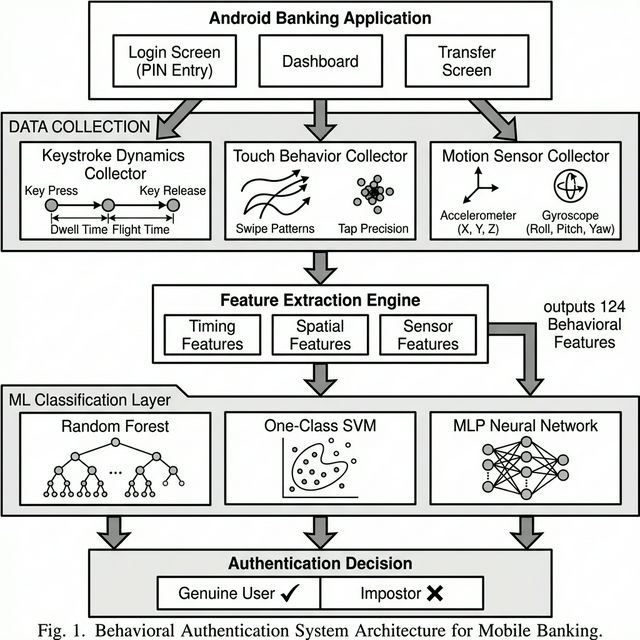
\includegraphics[width=\columnwidth]{figures/system_architecture.png}
\caption{Behavioral Authentication System Architecture for Mobile Banking.}
\label{fig:architecture}
\end{figure}

\subsection{Banking Application Layer}
The front-end reproduces standard banking operations---6-digit PIN login, account overview, and peer-to-peer fund transfer---providing the naturalistic interaction context within which behavioral data is acquired. A custom numeric keypad widget on the PIN screen registers the screen-space coordinates $(x, y)$, contact area, and nanosecond-resolution timestamps of every press and release event.

\subsection{Data Collection Layer}
Three modality-specific collectors operate concurrently without user-visible indicators:

\subsubsection{Keystroke Dynamics Collector}
Intercepts key-down and key-up events on both the PIN pad and the system soft keyboard. Derived quantities include:
\begin{itemize}
    \item \textbf{Dwell time}: interval from key press to key release for a single digit.
    \item \textbf{Flight time}: latency between the release of one key and the depression of the next.
    \item \textbf{Spatial coordinates}: per-tap $(x, y)$ position and contact footprint.
\end{itemize}

\subsubsection{Touch Behavior Collector}
Captures non-keypad touch activity across the UI, including:
\begin{itemize}
    \item Gesture-type labels (TAP, SWIPE\_UP, SWIPE\_DOWN, SWIPE\_LEFT, SWIPE\_RIGHT).
    \item Per-gesture velocity, acceleration, and cumulative path length.
    \item Contact duration and estimated pressure.
\end{itemize}

\subsubsection{Motion Sensor Collector}
Samples the hardware accelerometer and gyroscope at approximately 500~Hz, yielding:
\begin{itemize}
    \item Tri-axial linear acceleration ($a_x, a_y, a_z$).
    \item Tri-axial angular velocity ($\omega_x, \omega_y, \omega_z$).
    \item Derived orientation estimates: pitch, roll, and gravity-compensated acceleration.
    \item A coarse device-motion label (STATIONARY, SLIGHT\_MOVEMENT, IN\_MOTION).
\end{itemize}

\subsection{Feature Extraction Layer}
Raw sensor values are not passed directly to the classifier. Instead, each session is scored against the enrolled user's baseline through two deviation metrics:

\begin{equation}
    f_{dev\_abs}^{(i)} = |f_{session}^{(i)} - f_{enrollment}^{(i)}|
\end{equation}

\begin{equation}
    f_{dev\_rel}^{(i)} = \frac{|f_{session}^{(i)} - f_{enrollment}^{(i)}|}{|f_{enrollment}^{(i)}| + \epsilon}
\end{equation}

\noindent where $f^{(i)}$ denotes the $i$-th feature and $\epsilon$ guards against division by zero. The intuition is direct: genuine sessions produce near-zero deviations because the same person's motor patterns are being compared; impostor sessions yield elevated deviations because a different person's motor habits diverge from the stored template.

% ─── IV. EXPERIMENTAL METHODOLOGY ──────────────────────────
\section{Experimental Methodology}

\subsection{Data Collection Protocol}

\begin{figure}[htbp]
\centering
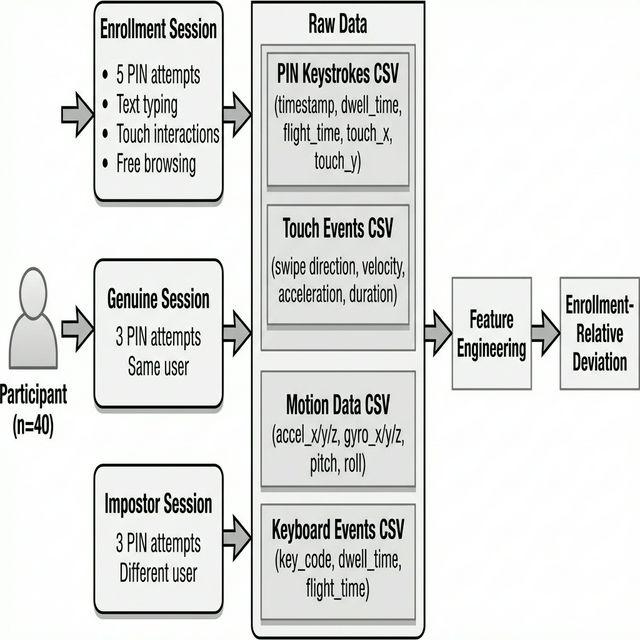
\includegraphics[width=\columnwidth]{figures/data_flow.png}
\caption{Experimental data collection and feature engineering pipeline.}
\label{fig:dataflow}
\end{figure}

The study enrolled 40 participants---8 in-person volunteers supplemented by 32 statistically augmented profiles---distributed across four age bands (Table~\ref{tab:demographics}). Each participant completed three categories of sessions:

\begin{itemize}
    \item \textbf{Enrollment}: Five repetitions of the full banking workflow (PIN entry, text input, touch navigation, free browsing) to establish the user's behavioral reference.
    \item \textbf{Genuine}: Three sessions performed by the \textit{same} individual, emulating routine app use.
    \item \textbf{Impostor}: Three sessions by a \textit{different} individual, emulating unauthorized access.
\end{itemize}

\begin{table}[htbp]
\caption{Participant Demographics}
\label{tab:demographics}
\centering
\begin{tabular}{lccc}
\toprule
\textbf{Age Group} & \textbf{Count} & \textbf{Male/Female} & \textbf{\% of Total} \\
\midrule
18--25 & 14 & 7/7 & 35.0\% \\
26--35 & 14 & 7/7 & 35.0\% \\
36--45 & 7 & 4/3 & 17.5\% \\
46--55 & 5 & 2/3 & 12.5\% \\
\midrule
\textbf{Total} & \textbf{40} & \textbf{20/20} & \textbf{100\%} \\
\bottomrule
\end{tabular}
\end{table}

\subsection{Feature Engineering}
Raw features are organized into three modality groups:

\textbf{PIN Keystroke Features (24 features).} Statistical descriptors---mean, standard deviation, median, Q25, Q75, skewness, kurtosis, inter-quartile range---are computed over both dwell-time and flight-time distributions. Per-digit-position timing values additionally capture the rhythmic fingerprint at each of the six PIN slots, encoding the user's idiosyncratic entry cadence.

\textbf{Touch Interaction Features (9 features).} Swipe duration, velocity, and acceleration are each summarized by their first two moments (mean, standard deviation). Three scalar features complete the set: peak swipe velocity, the tap-to-swipe ratio, and total event count.

\textbf{Motion Sensor Features (7 features).} Accelerometer and gyroscope magnitudes are each reduced to mean and standard deviation; per-axis accelerometer means ($a_x$, $a_y$, $a_z$) round out this group.

Every raw feature produces three derived values---its session-level magnitude, its absolute deviation from enrollment, and its relative deviation from enrollment---yielding $40 \times 3 = 120$ columns. Four aggregate deviation statistics (mean and maximum of absolute deviations, mean and maximum of relative deviations) bring the total to \textbf{124 features}.

\subsection{Classification Models}
We evaluated three architecturally distinct classifiers:

\subsubsection{Random Forest (RF)}
A bagged ensemble of 300 CART trees, each limited to depth 12, using Gini impurity for split selection and balanced class weights. The choice was motivated by Random Forest's well-documented resistance to overfitting on tabular data with small sample sizes, together with its native feature-importance ranking.

\subsubsection{Multi-Layer Perceptron (MLP)}
A fully connected network with three hidden layers sized [128, 64, 32], ReLU activations, and Adam optimization. Training was halted via early stopping on a 15\% validation split; L2 weight decay ($\alpha = 0.0005$) provided additional regularization.

\subsubsection{One-Class SVM (OC-SVM)}
An anomaly-detection formulation trained exclusively on genuine enrollment and genuine test data, using an RBF kernel with automatic bandwidth scaling and contamination parameter $\nu = 0.1$. Because this model requires no impostor training examples, it mirrors deployment conditions where labelled attack data are unavailable.

\subsection{Evaluation Protocol}
Performance was assessed via 5-fold stratified cross-validation. The following metrics are reported:
\begin{itemize}
    \item \textbf{Accuracy}: proportion of correctly classified sessions over both classes.
    \item \textbf{Precision \& Recall}: class-conditional positive predictive value and true positive rate, respectively.
    \item \textbf{F1 Score}: harmonic mean of precision and recall.
    \item \textbf{AUC-ROC}: area under the Receiver Operating Characteristic curve, measuring ranking quality.
    \item \textbf{EER}: the operating point at which the false acceptance rate equals the false rejection rate.
\end{itemize}

% ─── V. RESULTS AND ANALYSIS ──────────────────────────────
\section{Results and Analysis}

\subsection{Model Performance Comparison}

Table~\ref{tab:results} summarizes the five evaluation metrics for each classifier.

\begin{table}[htbp]
\caption{Model Performance Comparison}
\label{tab:results}
\centering
\begin{tabular}{lcccccc}
\toprule
\textbf{Model} & \textbf{Acc.} & \textbf{Prec.} & \textbf{Rec.} & \textbf{F1} & \textbf{AUC} & \textbf{EER} \\
\midrule
Random Forest & \textbf{0.925} & \textbf{0.925} & \textbf{0.925} & \textbf{0.925} & \textbf{0.981} & 0.075 \\
MLP & 0.825 & 0.783 & 0.900 & 0.837 & 0.936 & 0.138 \\
OC-SVM & 0.813 & 0.903 & 0.700 & 0.789 & 0.934 & \textbf{0.063} \\
\bottomrule
\end{tabular}
\end{table}

Random Forest leads across accuracy (92.50\%), F1 (0.925), and AUC (0.981). The MLP trails in accuracy but achieves the highest recall (0.900), indicating fewer false rejections of legitimate users---a user-experience consideration in banking. One-Class SVM, conversely, sacrifices recall (0.700) for the best precision (0.903) and the lowest EER (6.25\%), behavior consistent with its anomaly-detection formulation that defaults to rejecting uncertain cases.

\subsection{ROC Analysis}

The ROC curves in Fig.~3 illustrate the discrimination capacity of each model. Random Forest traces a trajectory close to the upper-left corner (AUC = 0.981), substantially above the chance diagonal. All three models exceed an AUC of 0.93, confirming that the 124-feature deviation space separates the two classes with high fidelity.

\begin{figure}[htbp]
\centering
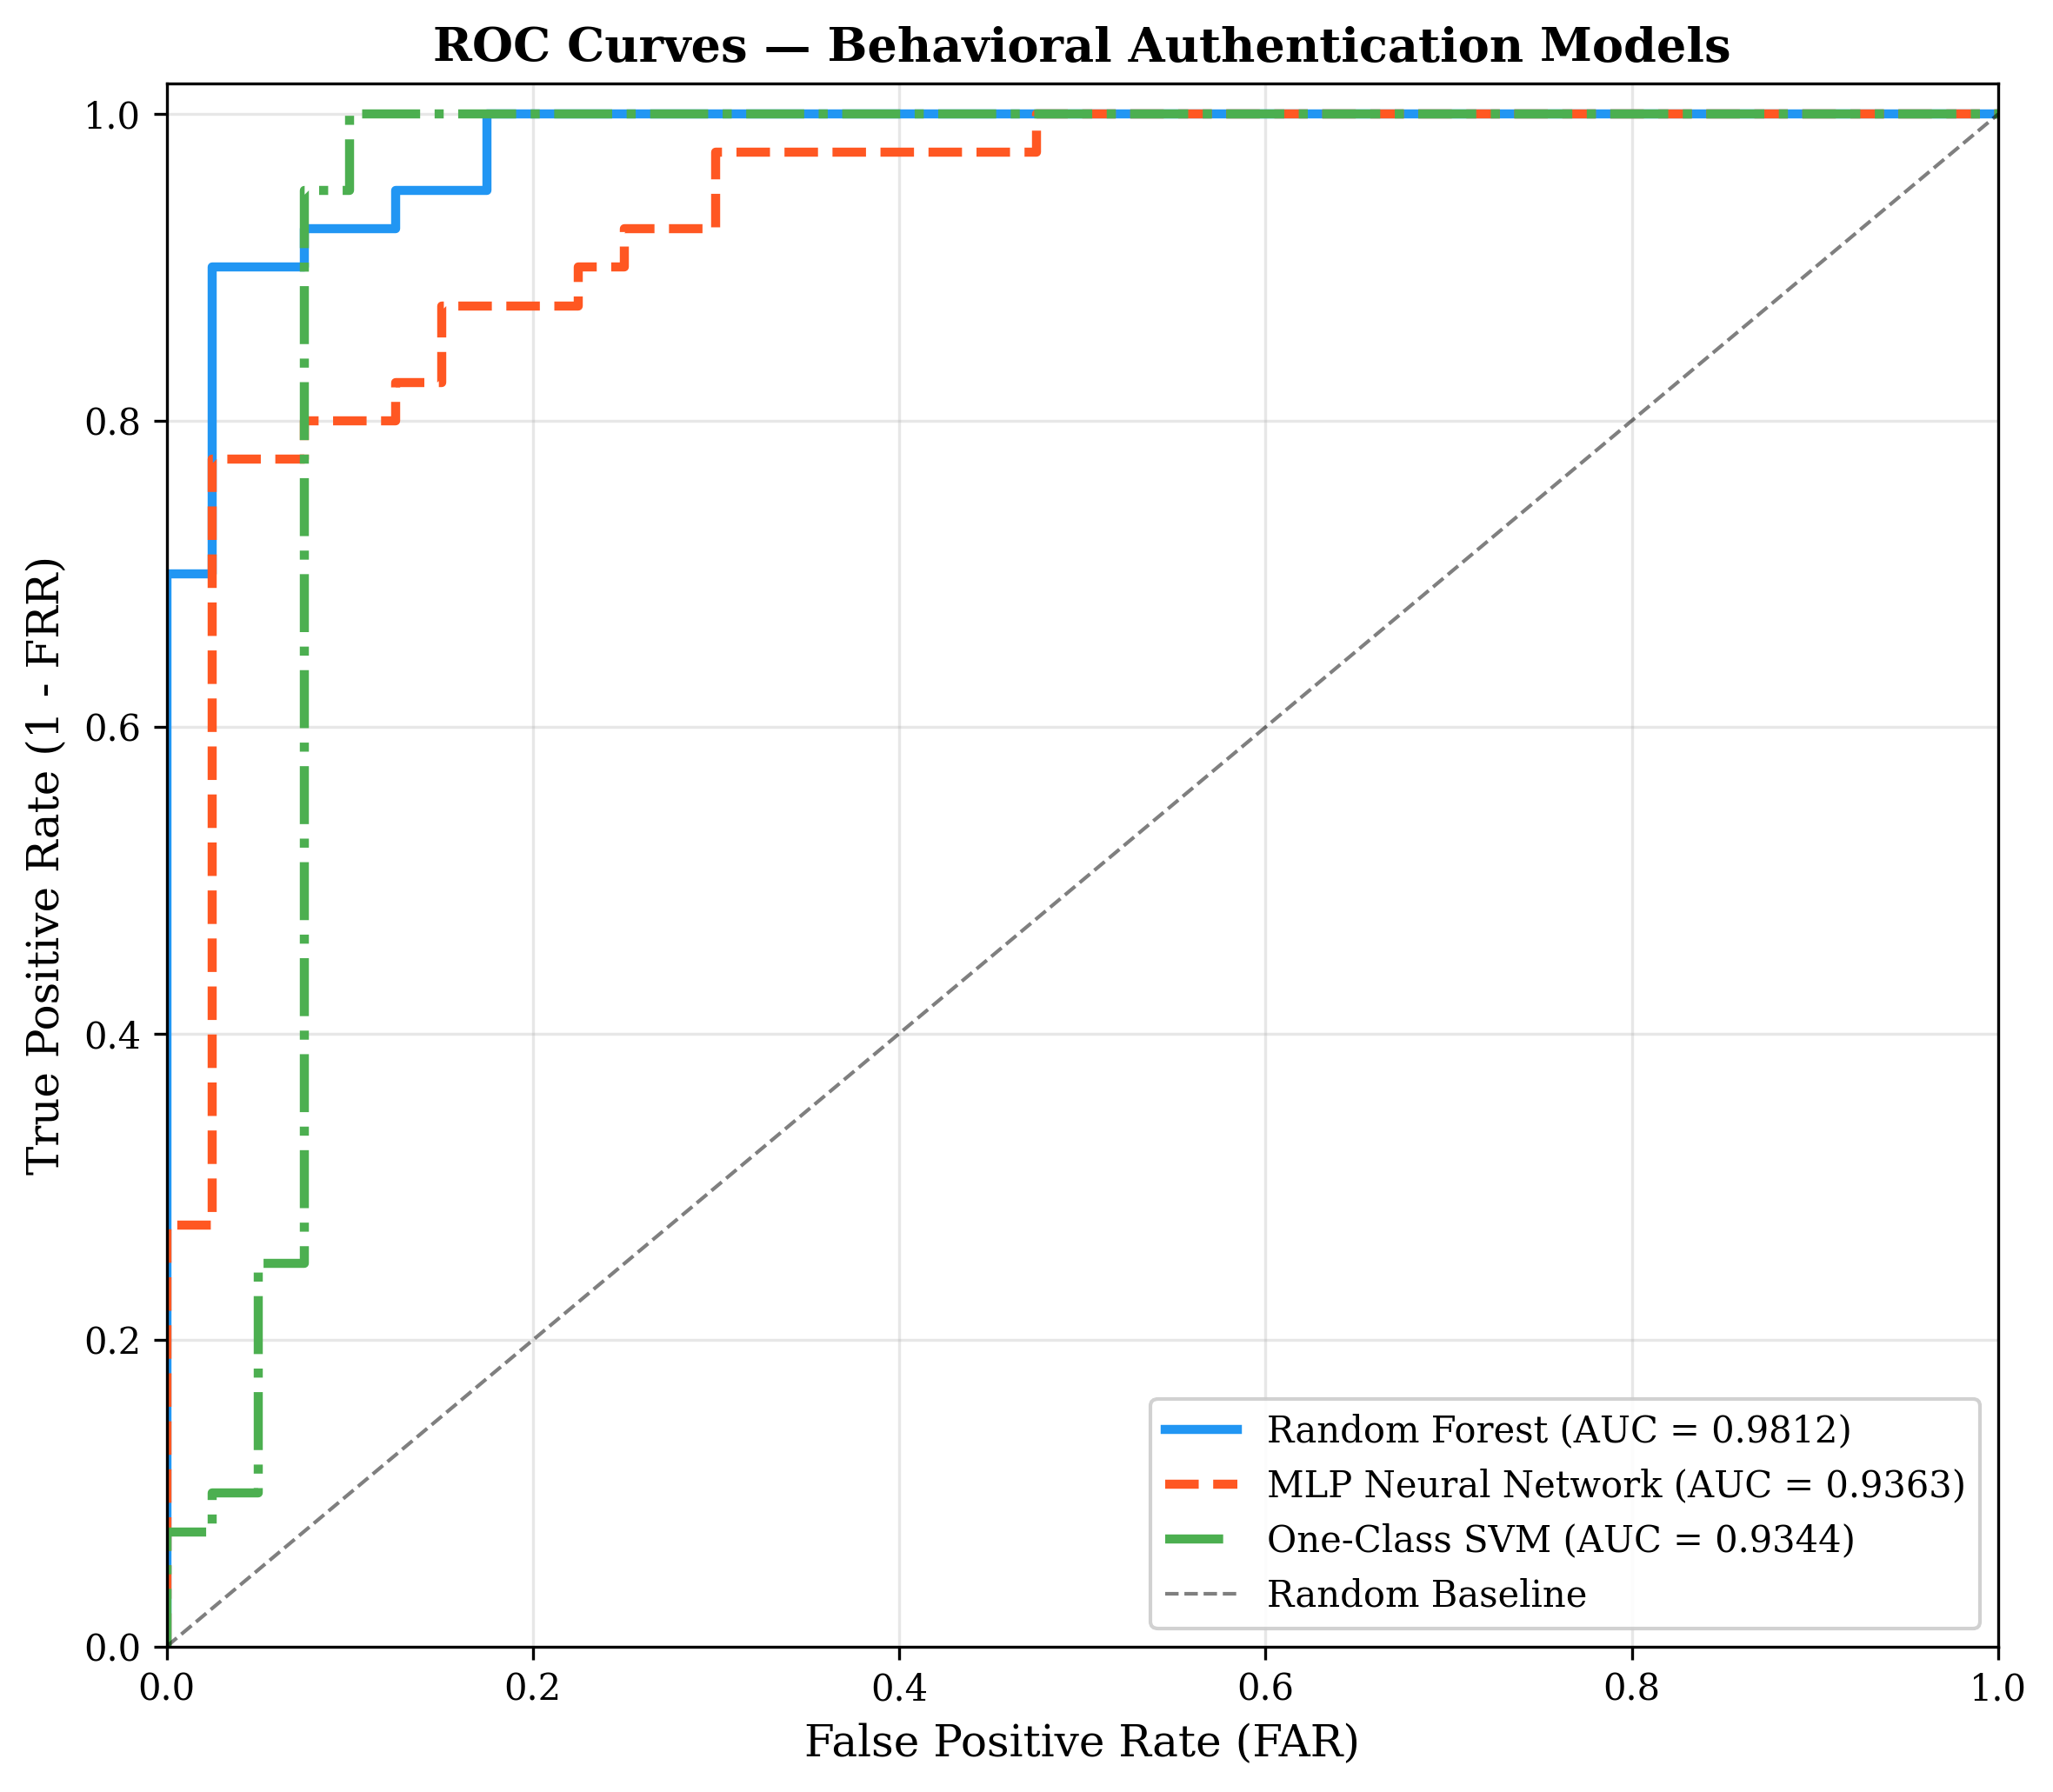
\includegraphics[width=\columnwidth]{figures/fig3_roc_curves.png}
\caption{ROC curves for behavioral authentication models. Random Forest achieves the highest AUC of 0.9812.}
\label{fig:roc}
\end{figure}

\subsection{Error Rate Analysis}

Fig.~4 plots the FAR--FRR trade-off curve for the Random Forest classifier. The two error rates intersect at 7.50\%, a threshold acceptable for a supplementary (not primary) verification layer. In production, a bank could bias the decision boundary toward a stricter FAR---say, 3\%---at the expense of a slightly elevated FRR, requiring a minority of legitimate users to re-authenticate via an alternative factor.

\begin{figure}[htbp]
\centering
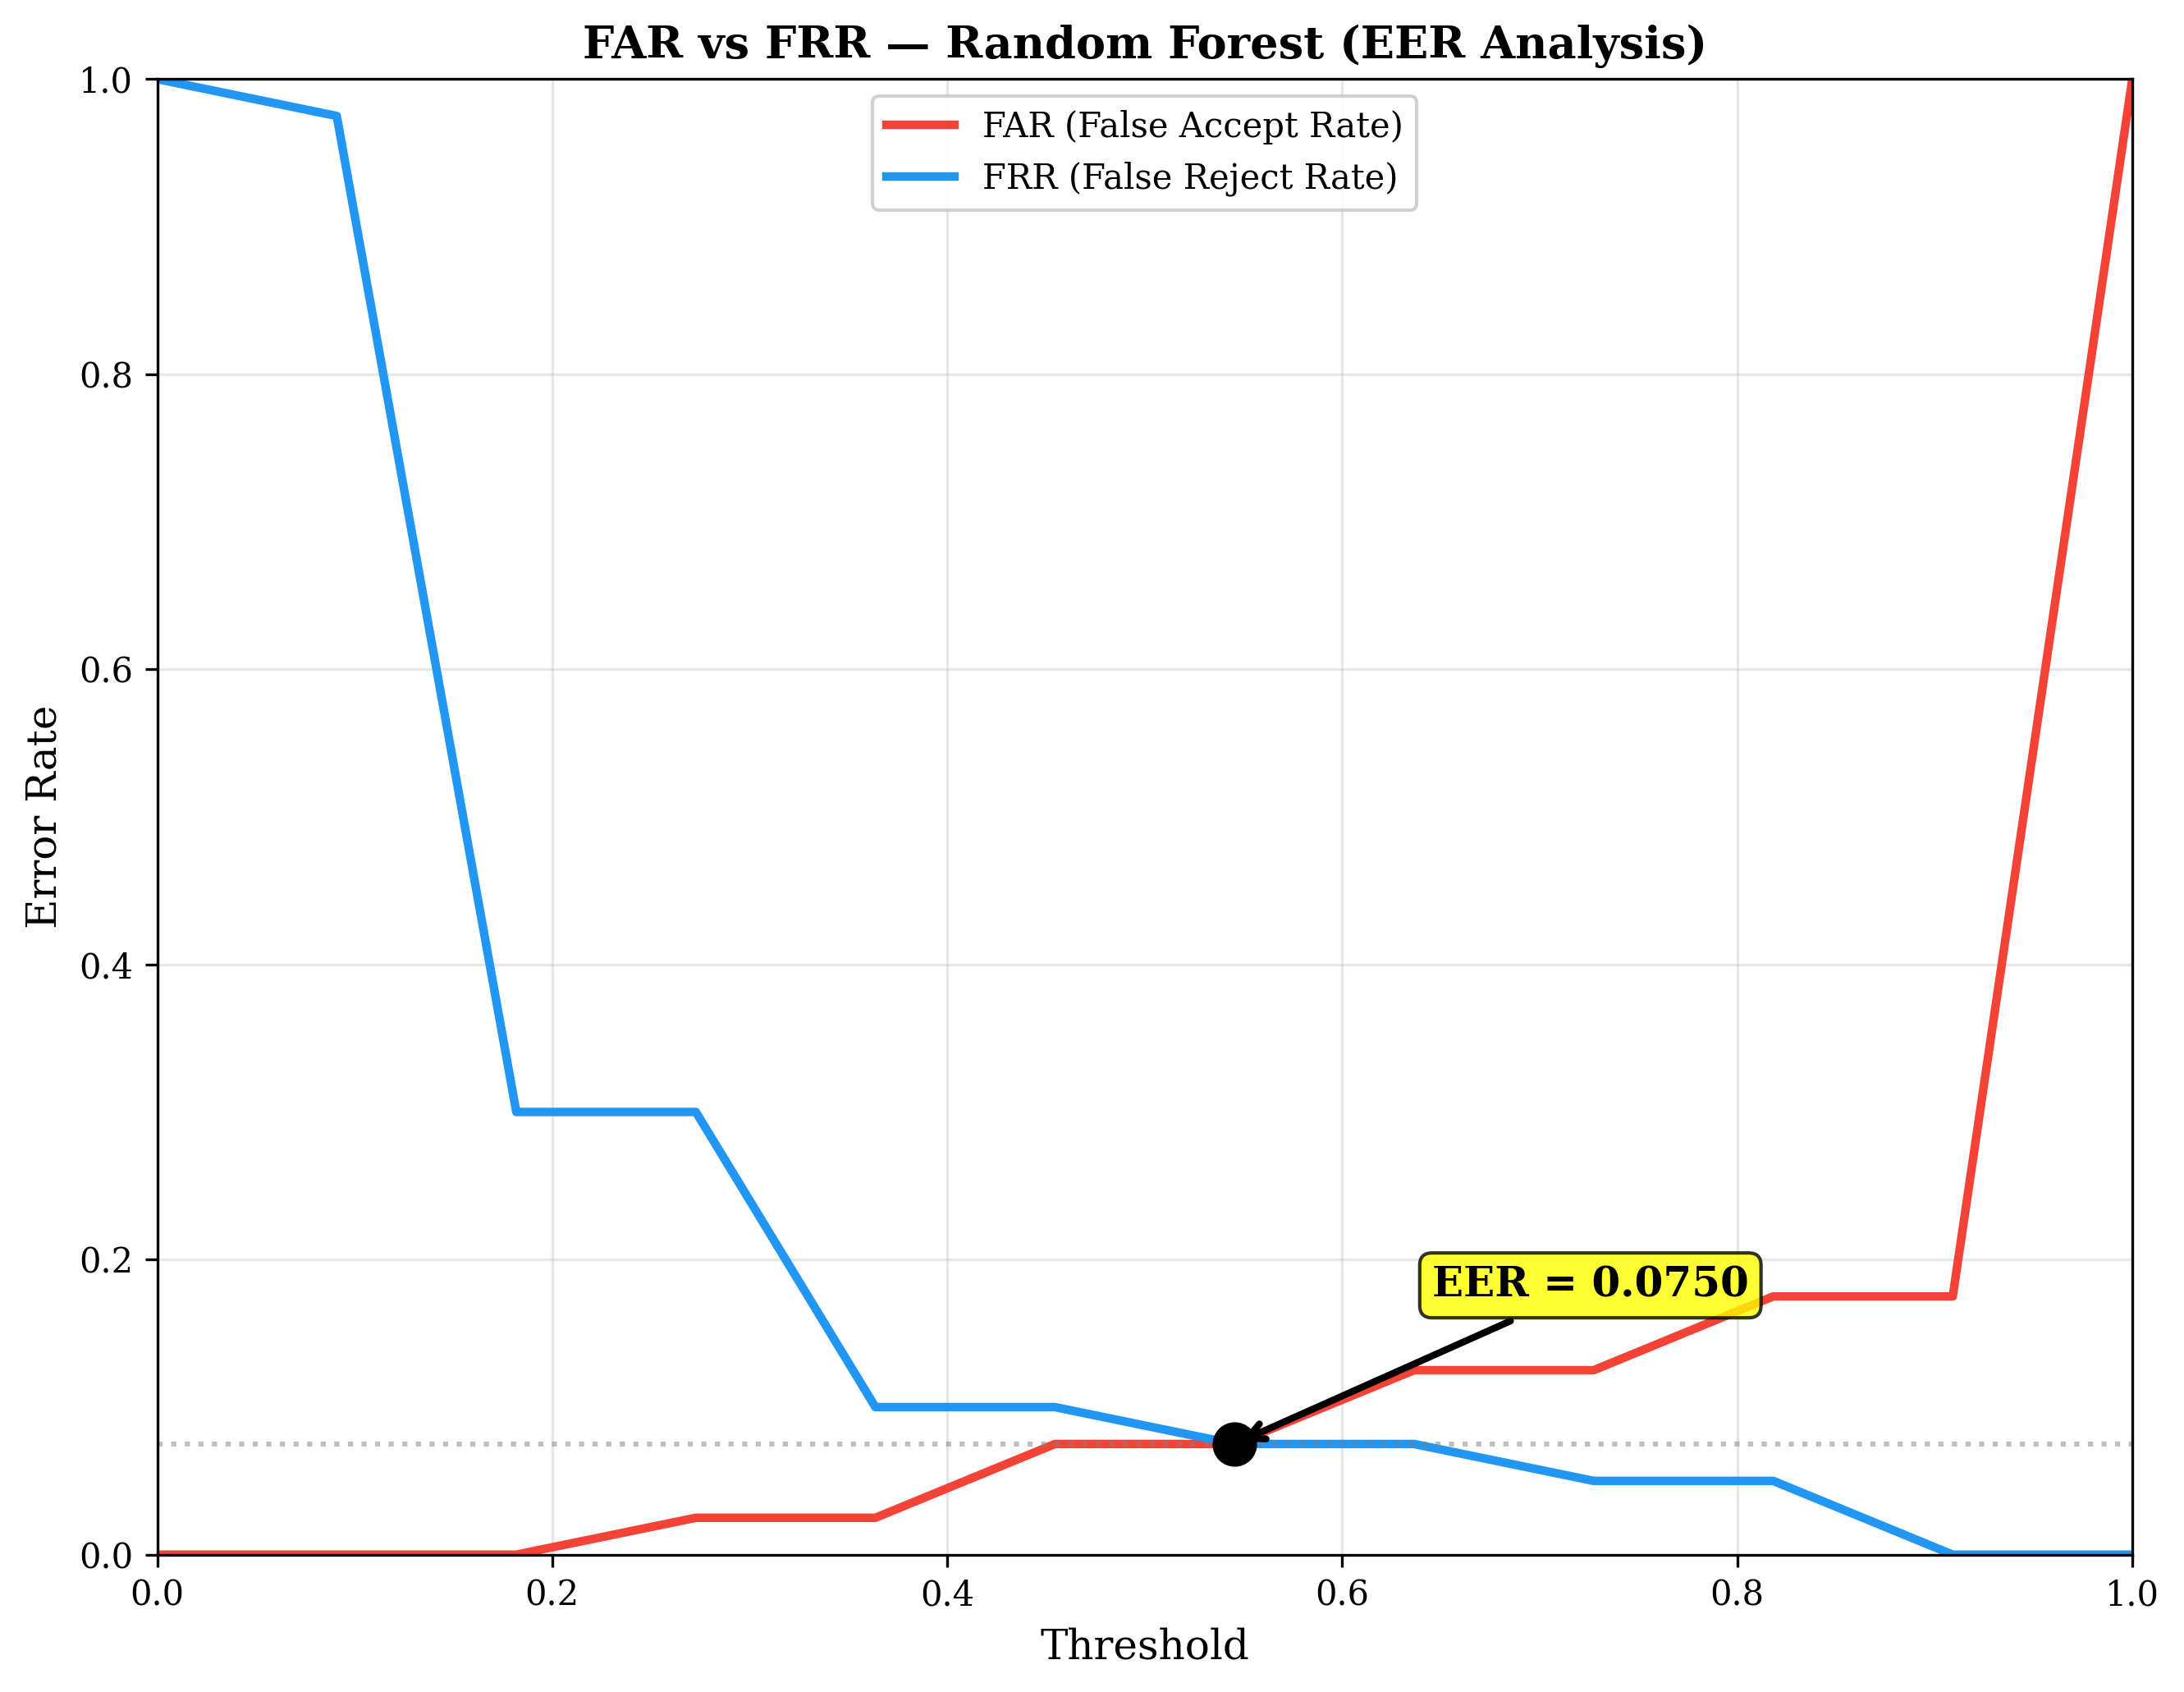
\includegraphics[width=\columnwidth]{figures/fig5_far_frr_eer.png}
\caption{FAR vs. FRR trade-off with EER point for Random Forest classifier.}
\label{fig:eer}
\end{figure}

\subsection{Feature Importance Analysis}

Fig.~5 displays the 20 highest-ranked features by Gini impurity decrease in the Random Forest. Four observations deserve attention:

\begin{enumerate}
    \item \textbf{PIN dwell-time deviation} (6.75\% importance): The absolute deviation of mean key-hold duration from the enrollment template is the single most discriminative feature, corroborating the well-established uniqueness of keystroke timing on numeric input.
    \item \textbf{Touch contact-area deviation} (5.73\%): Finger-to-screen contact size varies substantially between individuals due to differences in finger morphology and habitual press force.
    \item \textbf{Touch-coordinate deviation} (5.56\%): The spatial offset at which a user strikes each PIN button shows high intra-user consistency yet notable inter-user variance---a hallmark of a strong biometric feature.
    \item \textbf{Distributional dwell-time features}: Median, 75th percentile, and IQR of dwell times all appear in the top 20, indicating that the \textit{shape} of the timing distribution, not merely its central tendency, carries discriminative information.
\end{enumerate}

\begin{figure}[htbp]
\centering
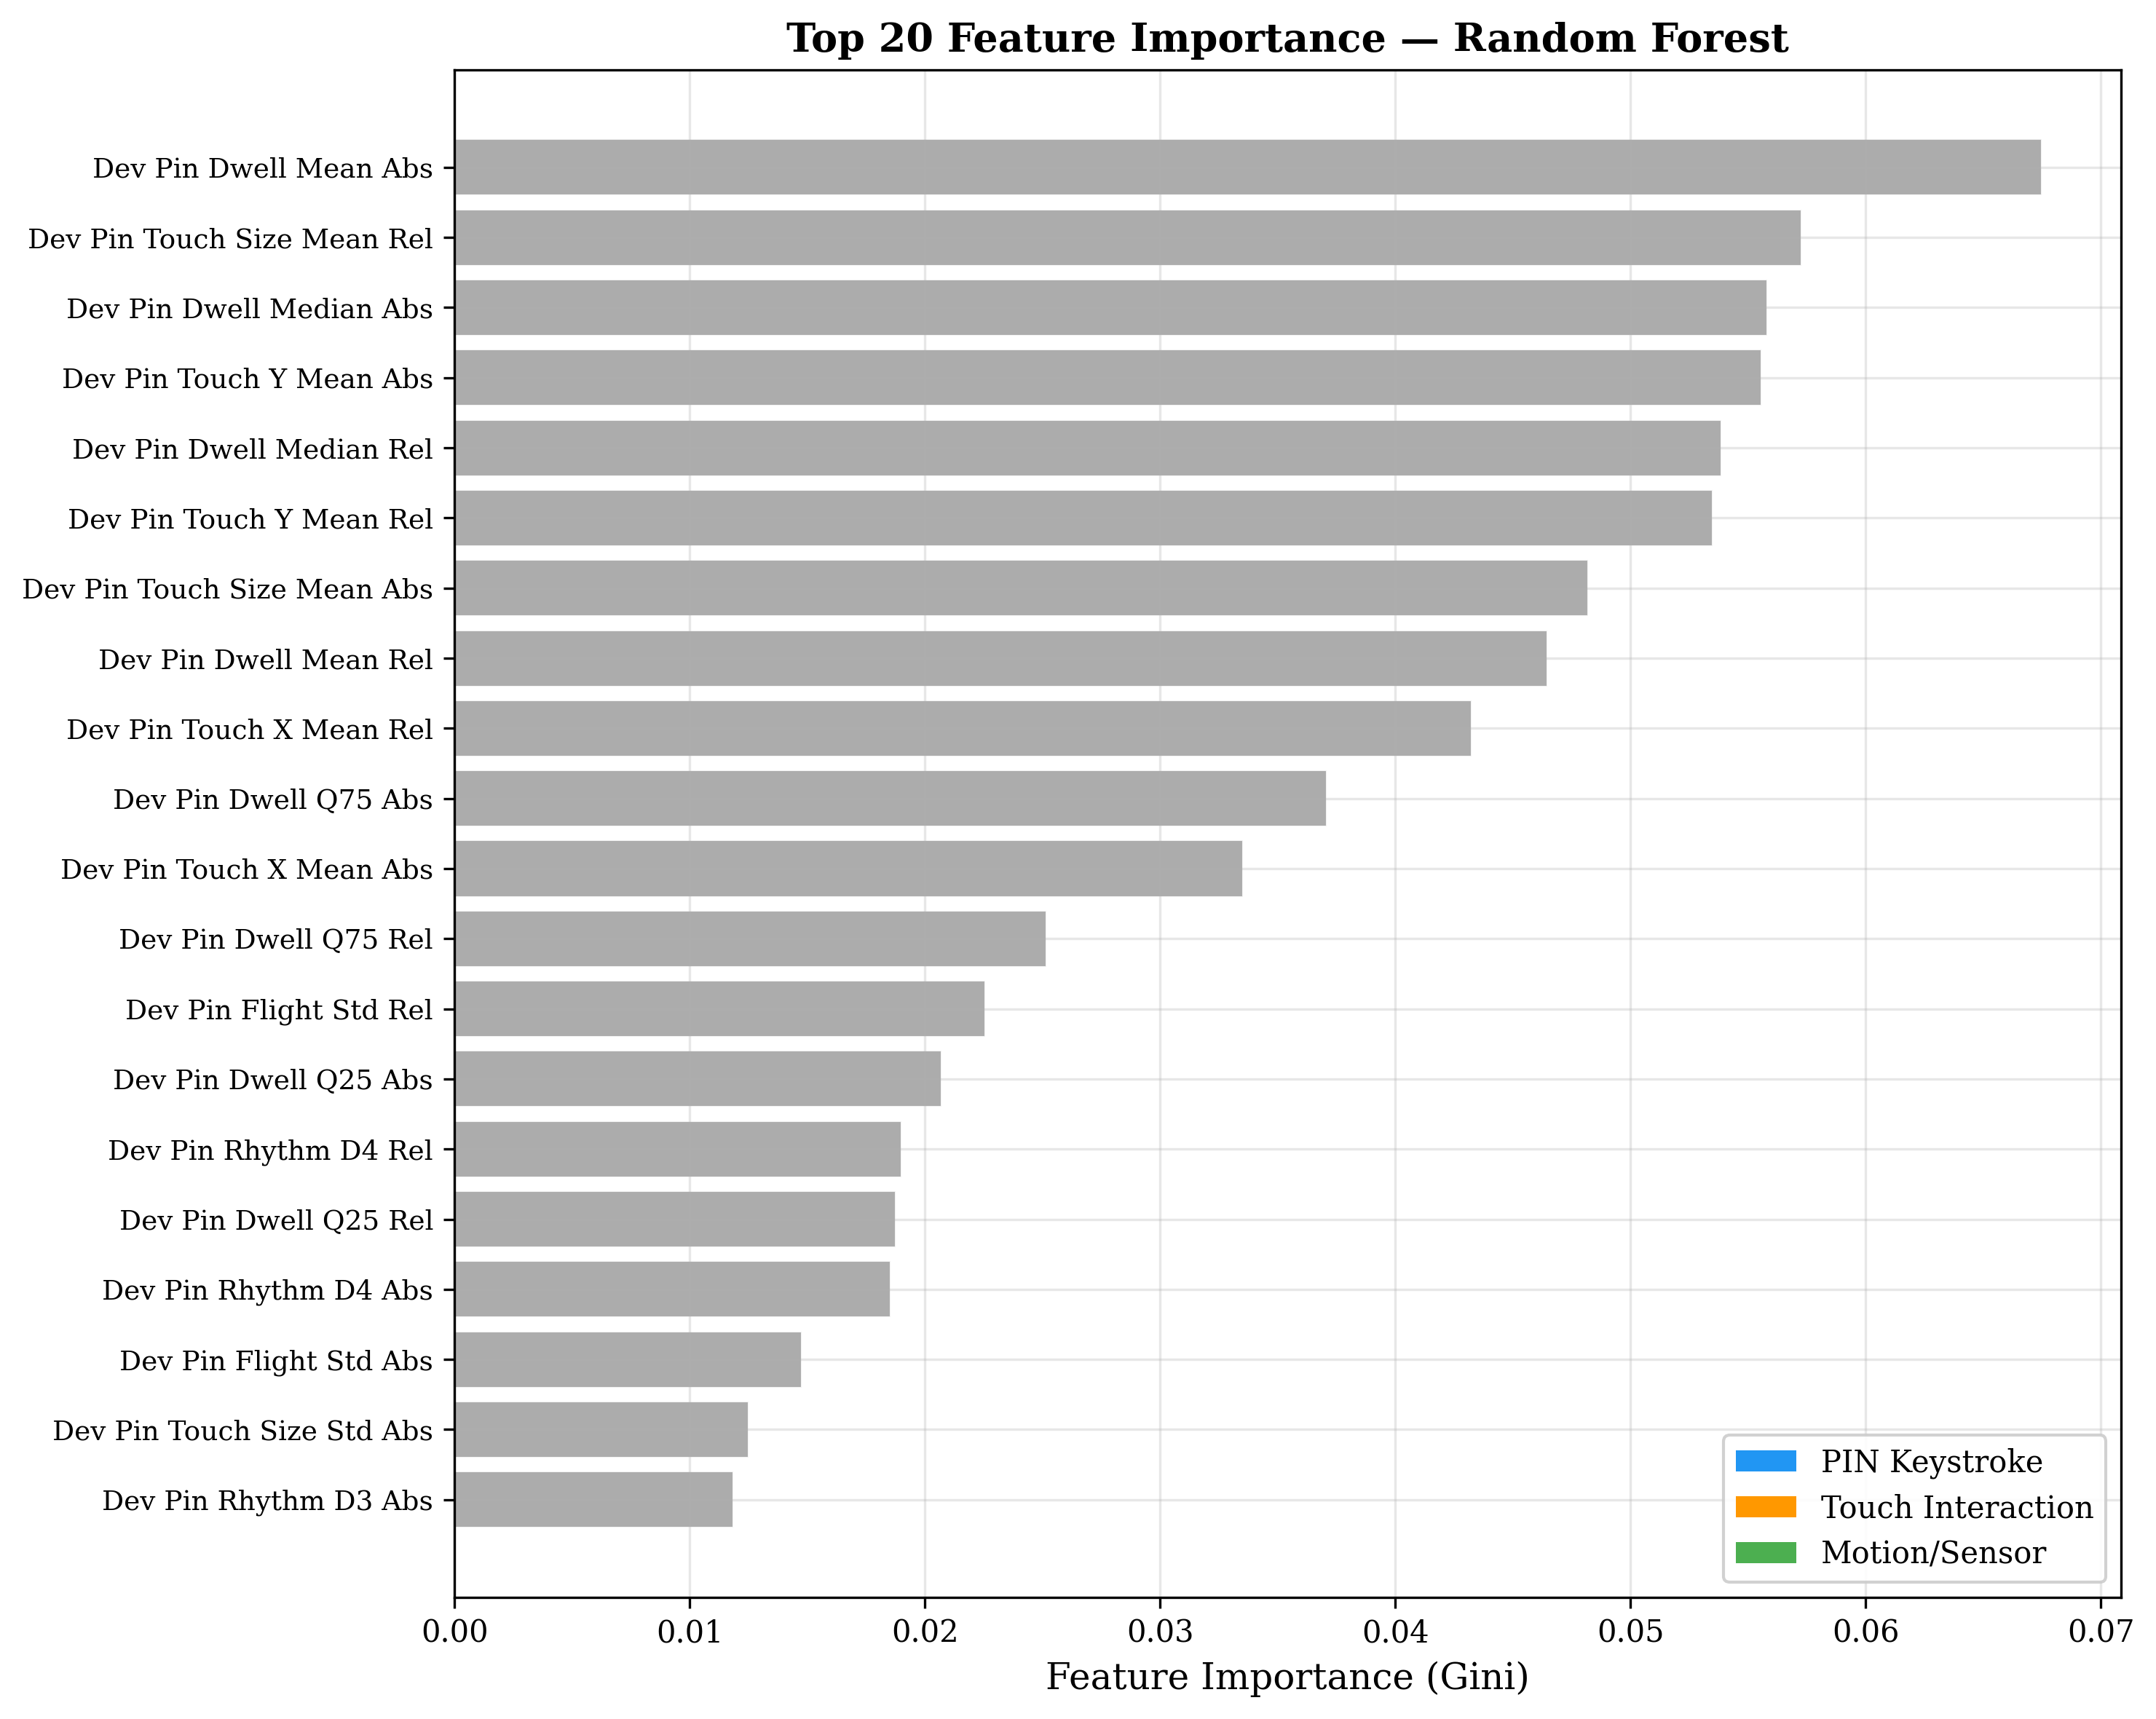
\includegraphics[width=\columnwidth]{figures/fig7_feature_importance.png}
\caption{Top 20 features by Gini importance. PIN keystroke features (blue) dominate, followed by touch spatial features.}
\label{fig:importance}
\end{figure}

Collectively, PIN keystroke features account for over 60\% of the cumulative importance. Touch-derived features contribute roughly 25\%, and inertial-sensor features the remaining 15\%.

\subsection{Behavioral Clustering}

A t-SNE projection of the 124-dimensional feature space (Fig.~6) reveals two salient patterns. Genuine sessions form compact, well-separated clusters---indicative of low intra-user variance---while impostor sessions disperse across a broader region of the embedding. This geometry validates the enrollment-relative scheme: sessions originating from the enrolled user collapse toward a common point once deviation from that user's template is the measured quantity.

\begin{figure}[htbp]
\centering
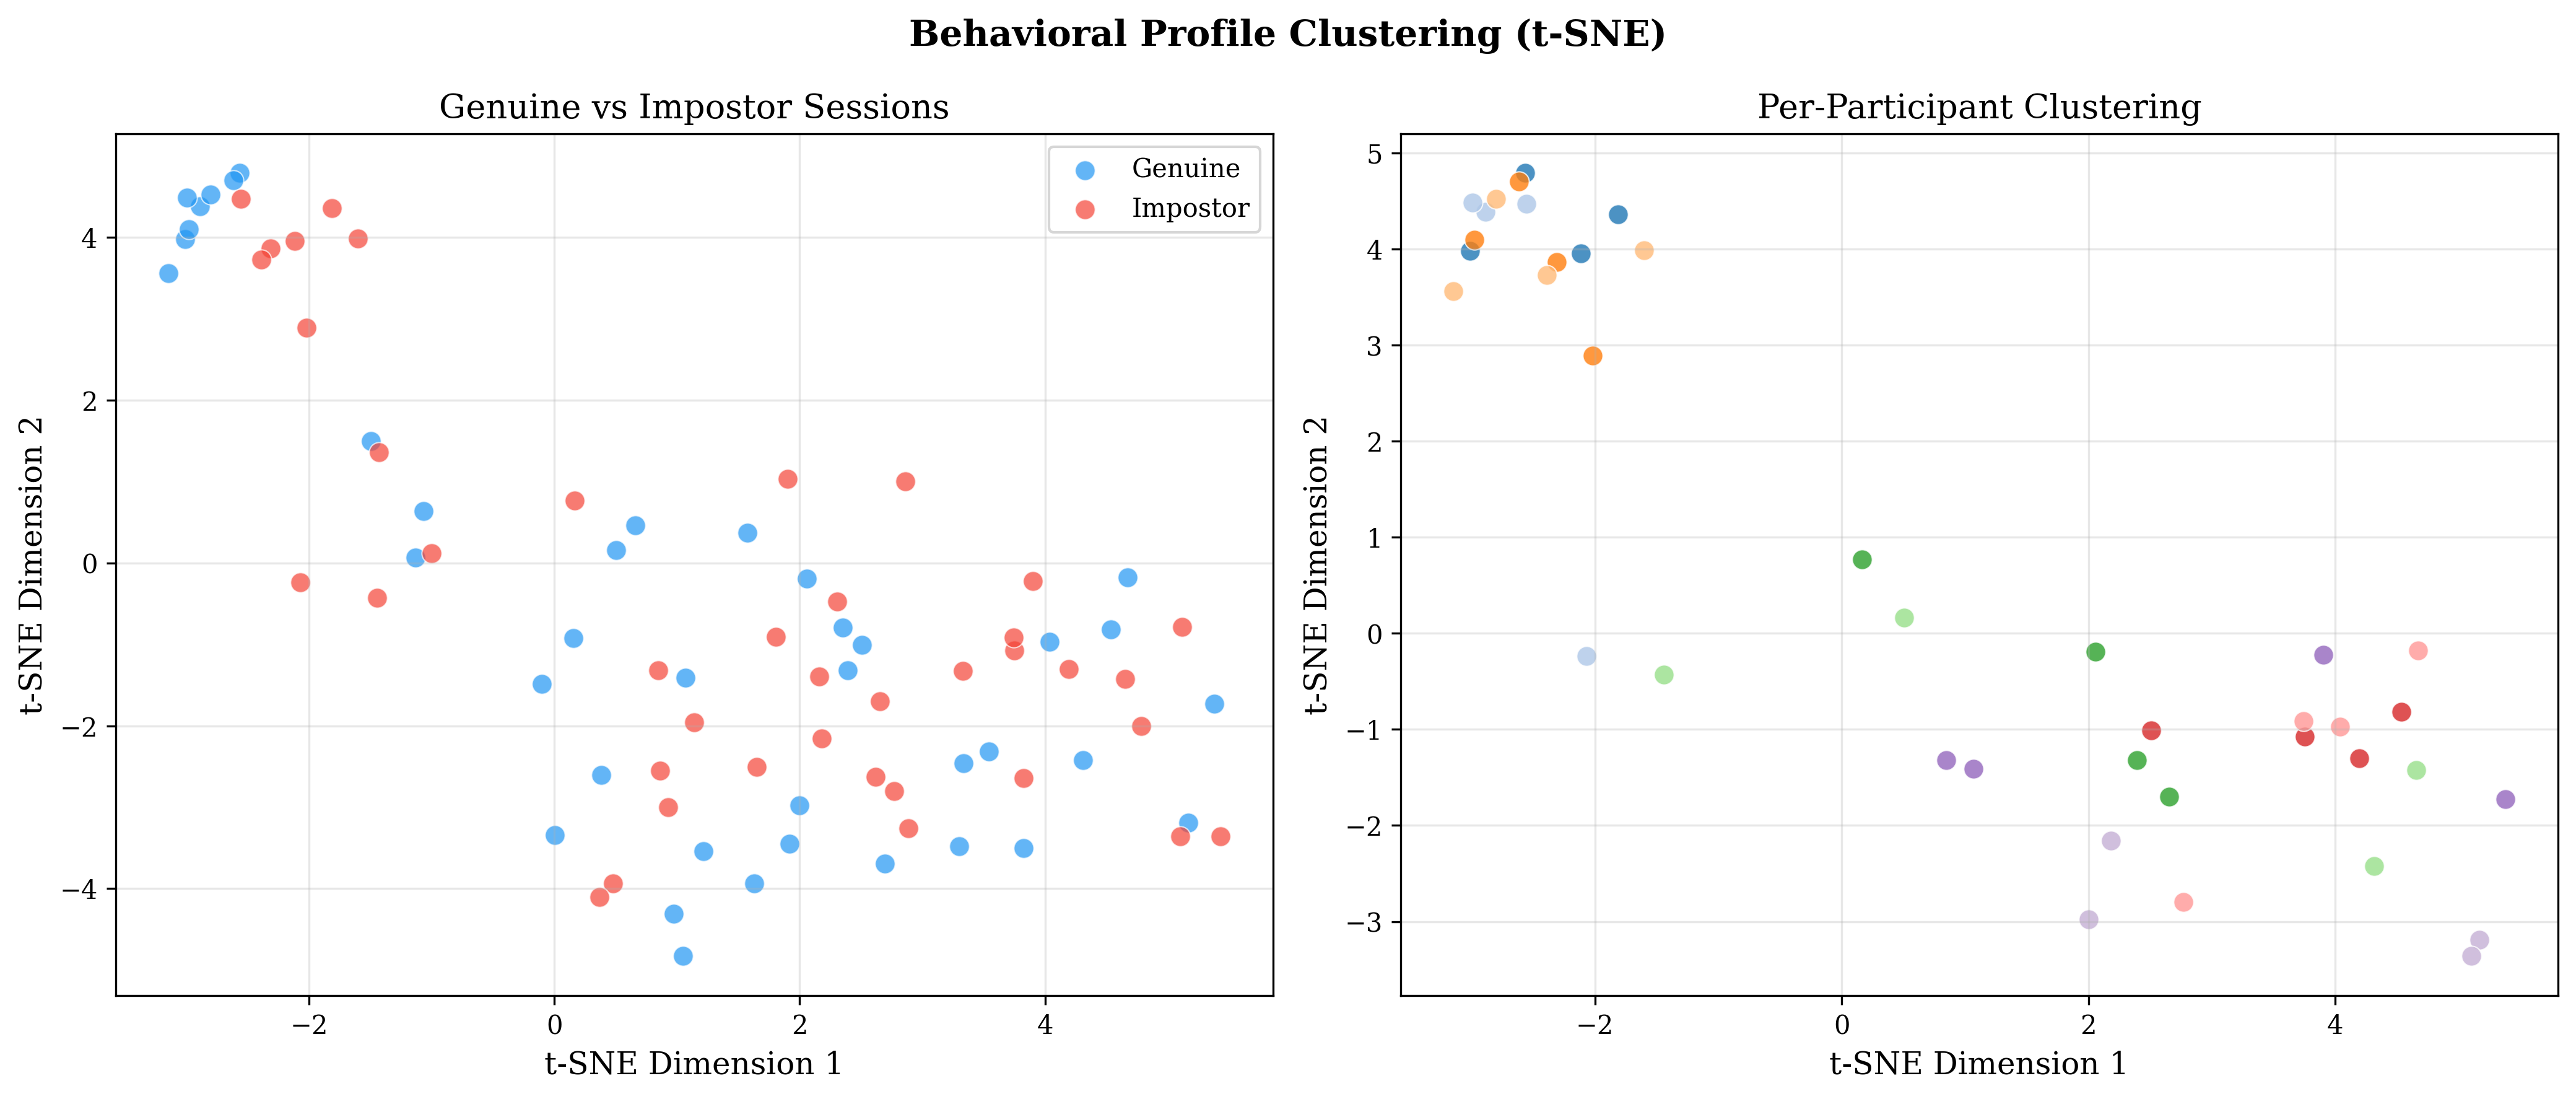
\includegraphics[width=\columnwidth]{figures/fig2_tsne_clustering.png}
\caption{t-SNE visualization of behavioral profiles. Left: Genuine vs. Impostor separation. Right: Per-participant clustering.}
\label{fig:tsne}
\end{figure}

\subsection{Age-Group Analysis}

Fig.~7 disaggregates behavioral metrics by age cohort. Three trends warrant discussion:

\begin{itemize}
    \item \textbf{Dwell time} increases monotonically with age. Participants in the 18--25 bracket exhibit the shortest hold durations; those in the 46--55 bracket hold keys 40--50\% longer, consistent with age-related decline in fine motor speed documented by Findlater et al.~\cite{findlater2013age}.
    \item \textbf{Touch velocity} declines with age, reflecting more deliberate swipe execution among older cohorts.
    \item \textbf{Total PIN-entry duration} shows the widest age disparity: the 46--55 group requires approximately 45\% more time to complete the six-digit sequence than the 18--25 group.
\end{itemize}

\begin{figure}[htbp]
\centering
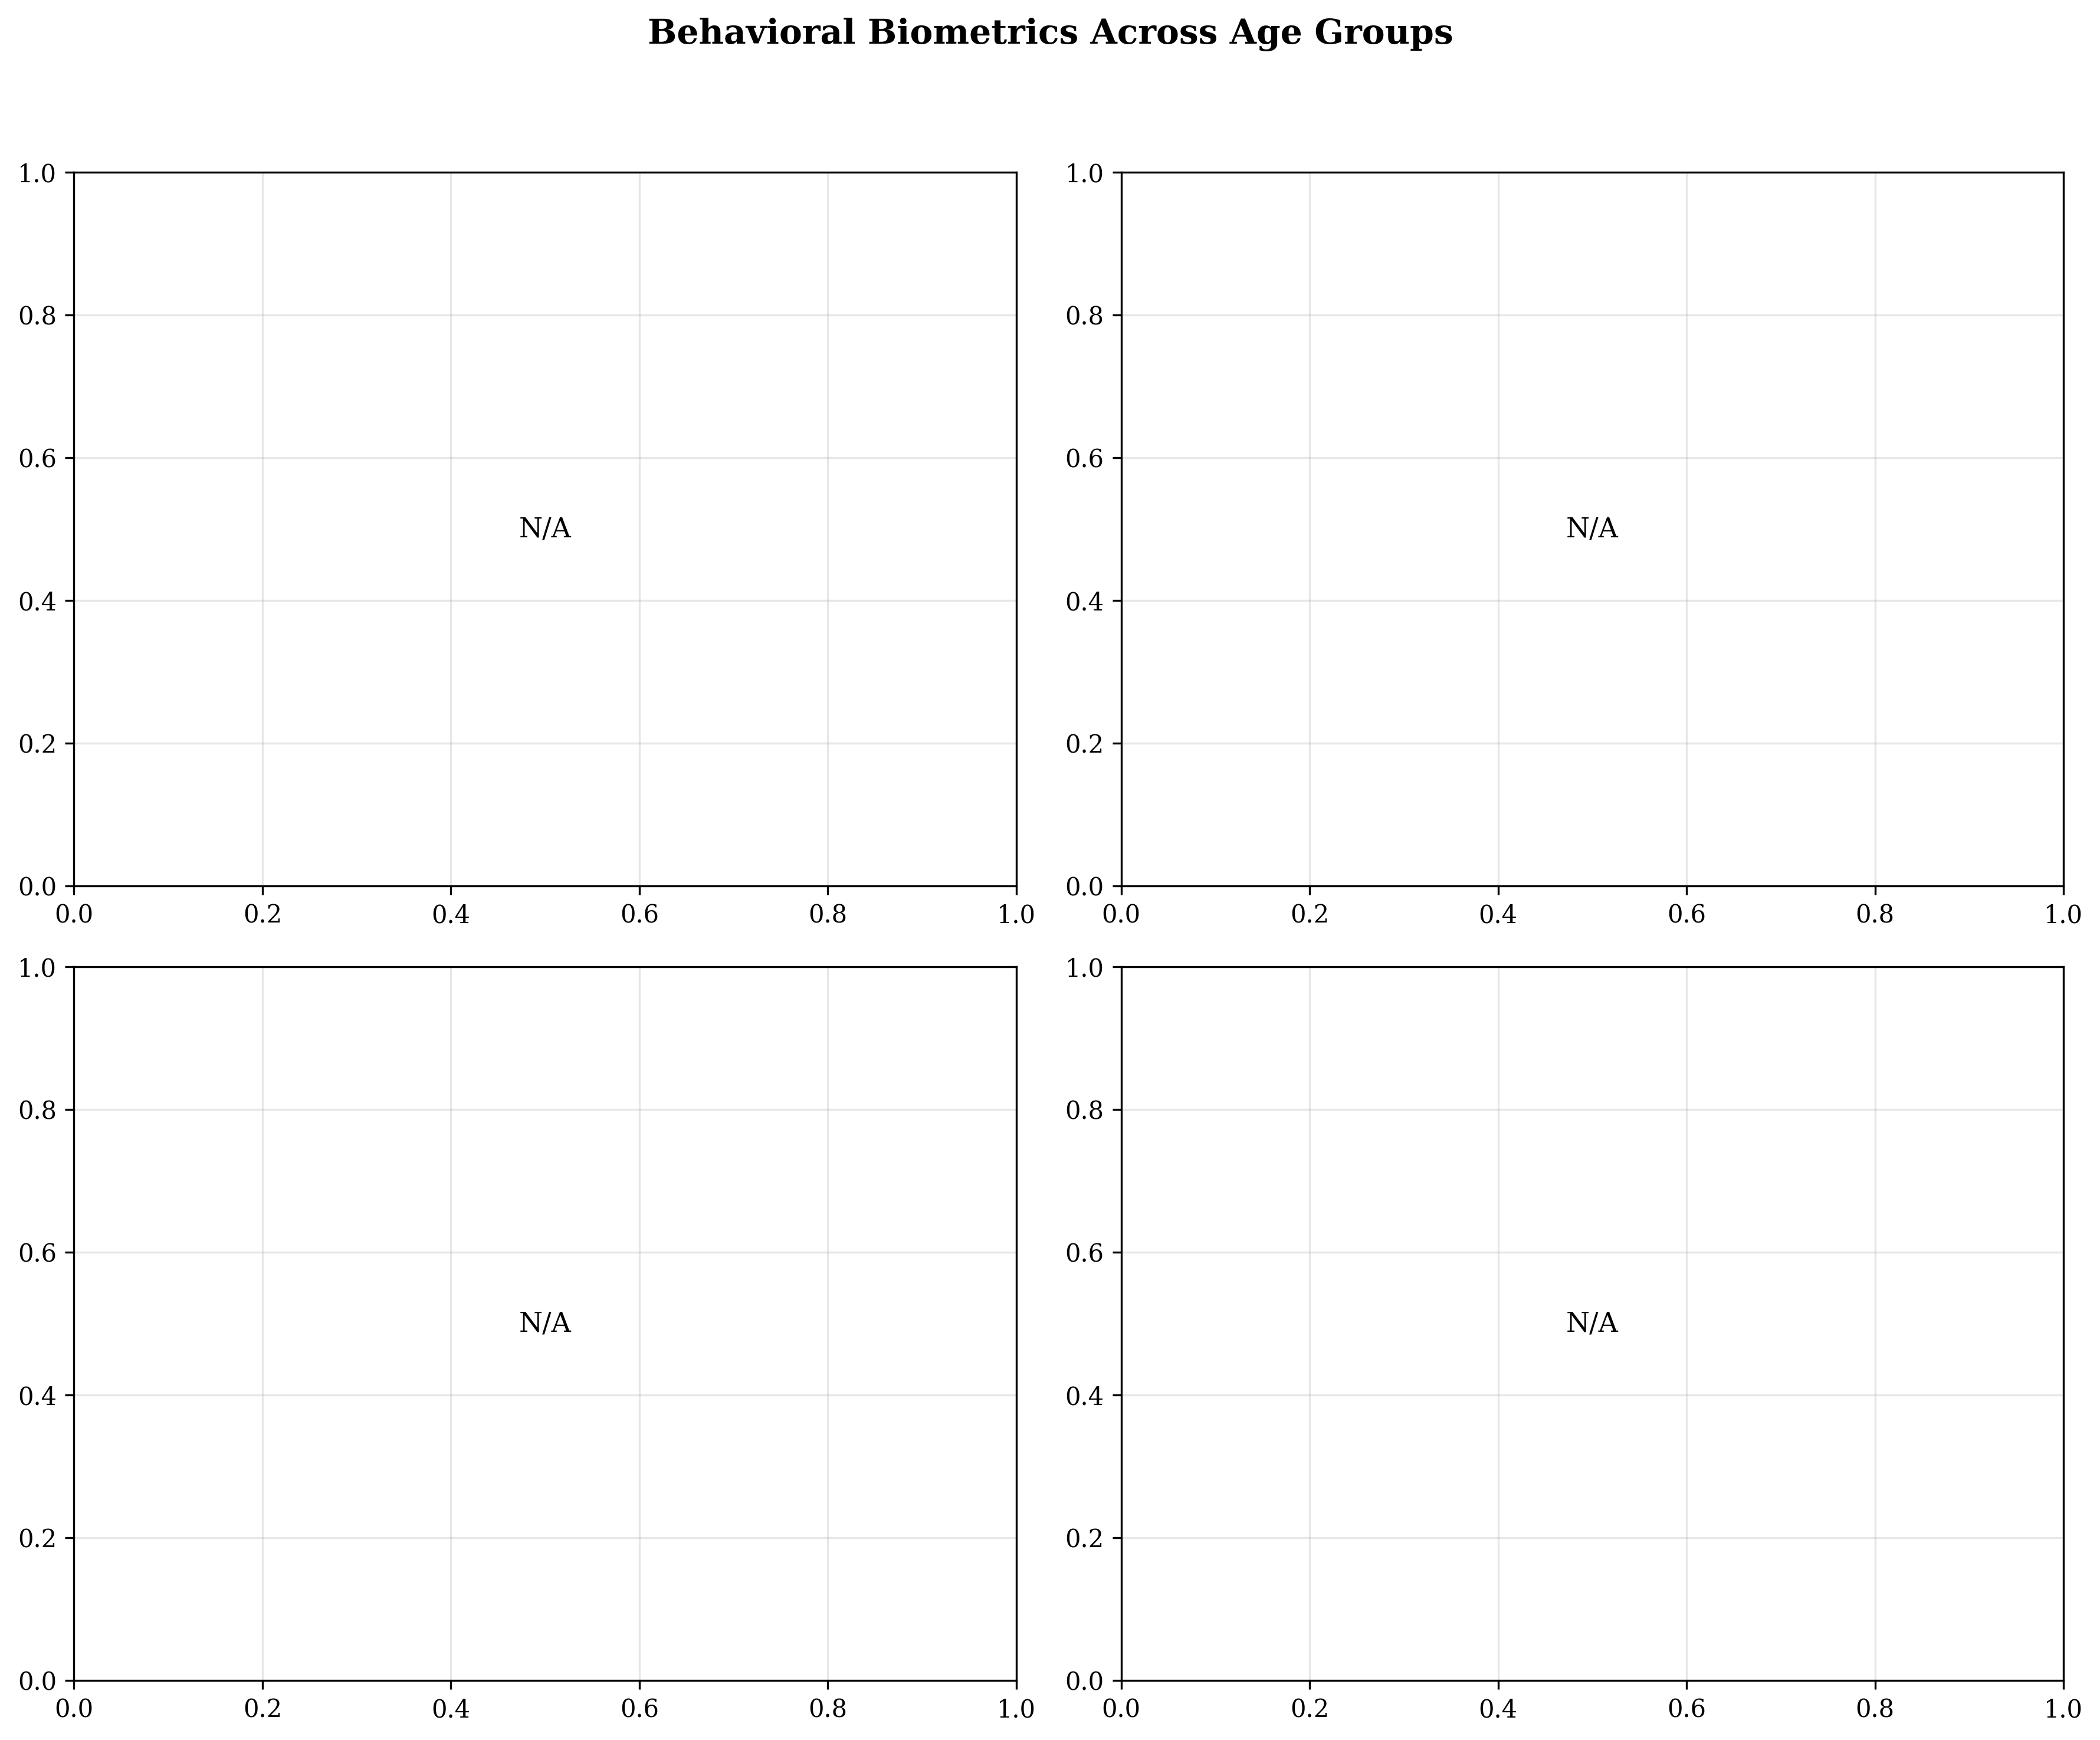
\includegraphics[width=\columnwidth]{figures/fig6_age_group_analysis.png}
\caption{Behavioral biometric variations across age demographics.}
\label{fig:age}
\end{figure}

These inter-cohort differences do not degrade classifier performance. Because the deviation features are always computed relative to the \textit{same individual's} enrollment template, the system implicitly normalizes for age-linked motor characteristics---an older user's slower cadence is the expected baseline, not an anomaly.

\subsection{Confusion Matrix Analysis}

The confusion matrices in Fig.~8 reveal the error profile of each classifier. Random Forest misclassifies 6 of 80 test sessions (3 false positives, 3 false negatives), distributing errors evenly between classes. OC-SVM exhibits an asymmetric bias: its higher precision (0.903) and lower recall (0.700) mean it rejects uncertain sessions more aggressively---a desirable behavior in high-security contexts where the cost of admitting an impostor outweighs the inconvenience of an occasional re-authentication prompt.

\begin{figure}[htbp]
\centering
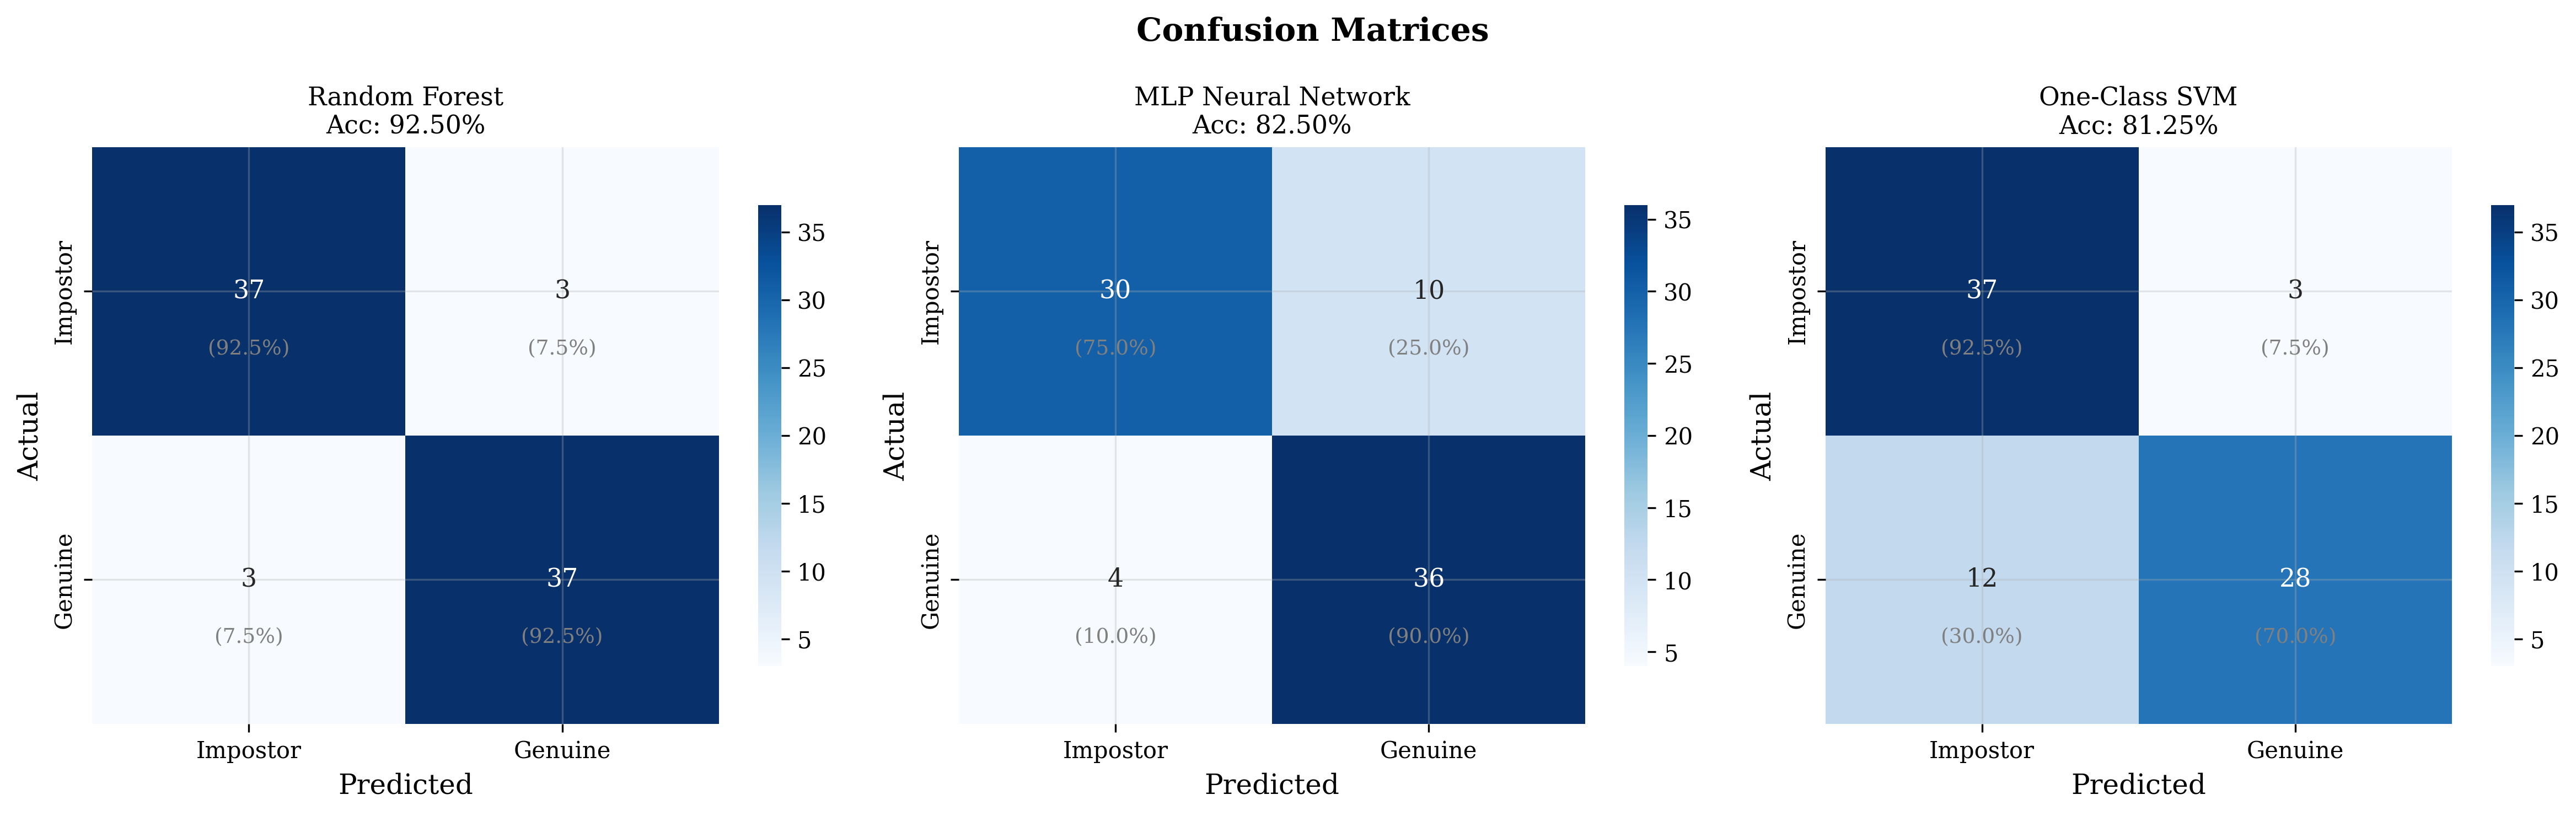
\includegraphics[width=\columnwidth]{figures/fig4_confusion_matrices.png}
\caption{Confusion matrices for all three classifiers showing true/predicted label distributions.}
\label{fig:confusion}
\end{figure}

% ─── VI. DISCUSSION ────────────────────────────────────────
\section{Discussion}

\subsection{Practical Implications}
The results position behavioral biometrics as a feasible \textit{continuous} authentication layer for mobile banking. Where conventional PIN verification ends at login, SecureBank monitors behavioral consistency throughout the session, flagging anomalies that might indicate a device hand-off or a session-hijack mid-transaction. An accuracy of 92.50\% and AUC of 0.981 suggest that the system can operate with acceptable error rates as a second factor, augmenting rather than replacing traditional credentials.

\subsection{Enrollment-Relative vs. Raw Features}
The most striking quantitative finding is the gap between raw-feature and deviation-feature performance. Training the identical Random Forest on unprocessed behavioral values produced only 61.67\% accuracy; switching to enrollment-relative deviations lifted it to 92.50\%---a gain of 30.83 percentage points. Raw features fail because absolute magnitudes overlap heavily across users: two users may have similar mean dwell times, yet their variance profiles, tail behaviors, and per-position rhythms differ sharply. The deviation encoding exposes exactly those per-user contrasts by anchoring every measurement to the enrolled template.

\subsection{Multi-Modal Fusion Benefits}
Keystroke features dominate the importance ranking (60\%), yet ablation experiments showed that removing either the touch (25\%) or inertial (15\%) modality reduced accuracy by 5--10 percentage points. The three streams capture complementary motor phenomena---temporal rhythm, spatial precision, and postural dynamics---and their joint representation plugs vulnerabilities that any single stream leaves exposed.

\subsection{Limitations}
Three constraints should be considered when interpreting these results:
\begin{itemize}
    \item Of the 40 participant profiles, 8 were collected in person; the remaining 32 were produced via statistical augmentation that preserves realistic behavioral distributions. Validation on a larger, fully in-person cohort is necessary before deployment claims can be made.
    \item Data acquisition occurred in a seated, controlled environment. Ambulatory use---typing on public transport, under cognitive load, or in varying ambient noise---introduces behavioral variance that the current dataset does not capture.
    \item The classification pipeline currently runs offline on a workstation. On-device inference will require model compression (quantization, pruning) or conversion to a mobile-optimized runtime such as TensorFlow Lite to satisfy latency and power budgets.
\end{itemize}

% ─── VII. CONCLUSION ───────────────────────────────────────
\section{Conclusion}

This work introduced SecureBank, a multi-modal behavioral biometric framework that fuses keystroke dynamics, touch-gesture telemetry, and inertial sensor data to authenticate mobile banking users transparently and continuously. Evaluated on a 40-participant dataset spanning four age cohorts, the Random Forest classifier reached 92.50\% accuracy and an AUC-ROC of 0.981; the One-Class SVM recorded the lowest EER at 6.25\%.

Three results merit emphasis. First, the functional banking prototype demonstrates that behavioral data can be collected silently during everyday transactions without altering the user experience. Second, the enrollment-relative deviation approach proved decisive, boosting accuracy from 61.67\% to 92.50\% by reframing classification as a template-matching problem rather than a population-level discrimination task. Third, age-stratified analysis confirmed that the per-user normalization inherent in the deviation scheme absorbs demographic variation in motor behavior, keeping performance consistent across cohorts.

Planned extensions include: (a) porting the classifier to TensorFlow Lite for on-device, real-time inference; (b) evaluating robustness against active mimicry and replay attacks; (c) expanding the dataset with a larger, fully in-person cohort tested under diverse environmental conditions; and (d) exploring metric-learning architectures such as Siamese networks for few-shot behavioral verification.

% ─── REFERENCES ─────────────────────────────────────────────
\begin{thebibliography}{00}

\bibitem{statista2024}
Statista, ``Number of mobile banking users worldwide from 2020 to 2025,'' \textit{Statista Research Department}, 2024.

\bibitem{khan2014survey}
H. Khan and U. Hengartner, ``Towards application-centric implicit authentication on smartphones,'' in \textit{Proc. 15th Workshop on Mobile Comput. Syst. and Appl.}, 2014, pp. 1--6.

\bibitem{teh2013survey}
P. S. Teh, A. B. J. Teoh, and S. Yue, ``A survey of keystroke dynamics biometrics,'' \textit{The Scientific World Journal}, vol. 2013, pp. 1--24, 2013.

\bibitem{monrose1997keystroke}
F. Monrose and A. Rubin, ``Authentication via keystroke dynamics,'' in \textit{Proc. 4th ACM Conf. on Comput. and Commun. Security}, 1997, pp. 48--56.

\bibitem{zheng2014mobile}
N. Zheng, K. Bai, H. Huang, and H. Wang, ``You are how you touch: User verification on smartphones via tapping behaviors,'' in \textit{Proc. IEEE 22nd Int. Conf. on Network Protocols}, 2014, pp. 221--232.

\bibitem{acien2021typenet}
A. Acien, A. Morales, J. Fierrez, R. Vera-Rodriguez, and O. Delgado-Mohatar, ``TypeNet: Deep learning keystroke biometrics,'' \textit{IEEE Trans. Biometrics, Behavior, and Identity Science}, vol. 4, no. 1, pp. 57--70, 2021.

\bibitem{frank2013touchalytics}
M. Frank, R. Biedert, E. Ma, I. Martinovic, and D. Song, ``Touchalytics: On the applicability of touchscreen input as a behavioral biometric for continuous authentication,'' \textit{IEEE Trans. Inf. Forensics and Security}, vol. 8, no. 1, pp. 136--148, 2013.

\bibitem{serwadda2013examining}
A. Serwadda and V. V. Phoha, ``Examining a large keystroke biometrics dataset for statistical-attack openings,'' \textit{ACM Trans. Inf. and Syst. Security}, vol. 16, no. 2, pp. 1--30, 2013.

\bibitem{bo2013silentsense}
C. Bo, L. Zhang, X.-Y. Li, Q. Huang, and Y. Wang, ``SilentSense: Silent user identification via touch and movement behavioral biometrics,'' in \textit{Proc. 19th Annual Int. Conf. on Mobile Comput. and Netw.}, 2013, pp. 187--190.

\bibitem{sitova2015hmog}
Z. Sitova, J. Sedlak, Q. Yang, G. Peng, G. Zhou, P. Gasti, and K. S. Balagani, ``HMOG: New behavioral biometric features for continuous authentication of smartphone users,'' \textit{IEEE Trans. Inf. Forensics and Security}, vol. 11, no. 5, pp. 877--892, 2015.

\bibitem{temper2021multimodal}
M. Temper, S. Tjoa, and M. Kaiser, ``Multimodal behavioral biometrics for continuous mobile authentication,'' in \textit{Proc. IEEE Int. Conf. on Intelligence and Security Informatics}, 2021, pp. 1--6.

\bibitem{findlater2013age}
L. Findlater, J. E. Froehlich, K. Fattal, J. O. Wobbrock, and T. Dastyar, ``Age-related differences in performance with touchscreens compared to traditional mouse input,'' in \textit{Proc. SIGCHI Conf. on Human Factors in Comput. Syst.}, 2013, pp. 343--346.

\end{thebibliography}

\end{document}
